\documentclass[review]{elsarticle}
\usepackage{comment}
\usepackage{url}
%
\usepackage[breaklinks]{hyperref}
\usepackage{breakurl}


\usepackage[ruled]{algorithm2e}

%\usepackage{lineno}
%\modulolinenumbers[5]

\journal{Optics Communications}

%%%%%%%%%%%%%%%%%%%%%%%
%% Elsevier bibliography styles
%%%%%%%%%%%%%%%%%%%%%%%
%% To change the style, put a % in front of the second line of the current style and
%% remove the % from the second line of the style you would like to use.
%%%%%%%%%%%%%%%%%%%%%%%

%% Numbered
%\bibliographystyle{model1-num-names}

%% Numbered without titles
%\bibliographystyle{model1a-num-names}

%% Harvard
%\bibliographystyle{model2-names.bst}\biboptions{authoryear}

%% Vancouver numbered
%\usepackage{numcompress}\bibliographystyle{model3-num-names}

%% Vancouver name/year
%\usepackage{numcompress}\bibliographystyle{model4-names}\biboptions{authoryear}

%% APA style
%\bibliographystyle{model5-names}\biboptions{authoryear}

%% AMA style
%\usepackage{numcompress}\bibliographystyle{model6-num-names}

%% `Elsevier LaTeX' style
\bibliographystyle{elsarticle-num}
%%%%%%%%%%%%%%%%%%%%%%%
\usepackage[]{graphicx}

%%%%%%%%%%%%%%%%%%%%%%%%%%%%%%%%%%%%%%%%%%%%%%%%%%%%%%%%%%%%%%%%%%%%%%%%%%%%%%%%%%

\usepackage[svgnames]{xcolor} % Enabling colors by their 'svgnames'

\usepackage{amsmath}
\usepackage{amsfonts}
\usepackage{amssymb}
%%%%%%%%%%%%%%%%%%%%%%%%%%%%%%%%%%%%%%%%%%%%%%%%%%%%%%%%%%%%%%%%%%%%%%%%%%%%%%%%%%

 
\begin{document} 

\begin{frontmatter}

\title{Sound as a Qualitative Biospeckle Index Interpretation in the Biospeckle Laser Analysis}
%\tnotetext[mytitlenote]{Fully documented templates are available in the 
%elsarticle package on \href{http://www.ctan.org/tex-archive/macros/latex/contrib/elsarticle}{CTAN}.}



% Group authors per affiliation:
\author{-------- ------- ------}
\author{-------- ------- ------}



% \author{Fernando Pujaico Rivera\fnref{myfootnote2}}
% \author{Roberto Alves Braga Jr.\fnref{myfootnote1}}
% \address{University Federal of Lavras, Lavras, Brazil}
% \fntext[myfootnote2]{201518201@posgrad.ufla.br}
% \fntext[myfootnote1]{robertobraga@deg.ufla.br }


\begin{abstract}
In this article will be studied two biospeckle analysis methods, in both cases
a sound representation of biospeckle analysis will be presented. The first case
uses single frequency band model, so that all the spectral information is interpreted by
an unique biospeckle index. In the second case a multi frequency band interpretation
is used and the signal is separated in $N$ frequency bands, and in these, biospeckle
indexes are calculated; finally it is made a sound interpretation of these results.
Results of analysis show that these methods are a good \textcolor{blue}{qualitative and relative} 
interpretation of the biospeckle analysis, providing a fast understanding of the state the
biospeckle activity in the points analyzed.
\end{abstract}

\begin{keyword}
Biospeckle laser \sep 
Biospeckle index \sep 
Biospeckle signal\sep 
Biological activity \sep
Dynamic speckle \sep  
Backscattering.
\end{keyword}

\end{frontmatter}

\linenumbers

%%%%%%%%%%%%%%%%%%%%%%%%%%%%%%%%%%%%%%%%%%%%%%%%%%%%%%%%%%%%%%%%%%%%%%%%%%%%%%%%%%%%%%%%%
%%%%%%%%%%%%%%%%%%%%%%%%%%%%%%%%%%%%%%%%%%%%%%%%%%%%%%%%%%%%%%%%%%%%%%%%%%%%%%%%%%%%%%%%%
\section{Introduction}
The biospeckle laser analysis has presented as a versatile tool in the analysis of
biological activity in many types of biological materials; with the grow of the demand in 
the use of this technique, also are required new methods of present the result. Thus, they
are well known in the literature numerical ans graphic methods \cite{avd,Nothdurft:05},
in the case of numerical methods these are a good quantitative form of 
differentiate between two distinct levels of biospeckle activity, by other side in the case
of graphic methods these have showed efficient to show qualitatively the level biospeckle activity 
in each point of an analysis region to the case of a unique analyzed frequency band,
already in the multi frequency band case the representation of data 
tends to be more complex to interpret. 
Thus, born the necessity of design a new form of to show qualitatively the level biospeckle 
activity, that will be easy to interpret, both in the single frequency band case and in 
the multi frequency band case. Thereby, in this work is proposed a 
qualitative biospeckle index interpretation using a sound.

%%%%%%%%%%%%%%%%%%%%%%%%%%%%%%%%%%%%%%%%%%%%%%%%%%%%%%%%%%%%%%%%%%%%%%%%%%%%%%%%%%%%%%%%%
%%%%%%%%%%%%%%%%%%%%%%%%%%%%%%%%%%%%%%%%%%%%%%%%%%%%%%%%%%%%%%%%%%%%%%%%%%%%%%%%%%%%%%%%%
\section{System description}

The materials used in the tests presented in this work, 
consist of a laser with a wavelength of 632 nm (red color), pointing to
a coffee seed in germinating process, the speckle patter produced is acquired by
a digital camera connected to a personal computer with the Octave software \cite{OCTAVE} installed;
additionally was installed over Octave, the
biospeckle laser tool library \cite{BSLTLBOOK,BSLTL}.
The acquired images were sampled with a rate of $0.08$s, equivalent to a 
sampling frequency of $F_s=12.5hz$ into 8 bits format; where,
the images have a size of 448$\times$448 pixels (lines and columns respectively), being
a total of $M=128$ images, 
\begin{figure}[ht!]
\centering
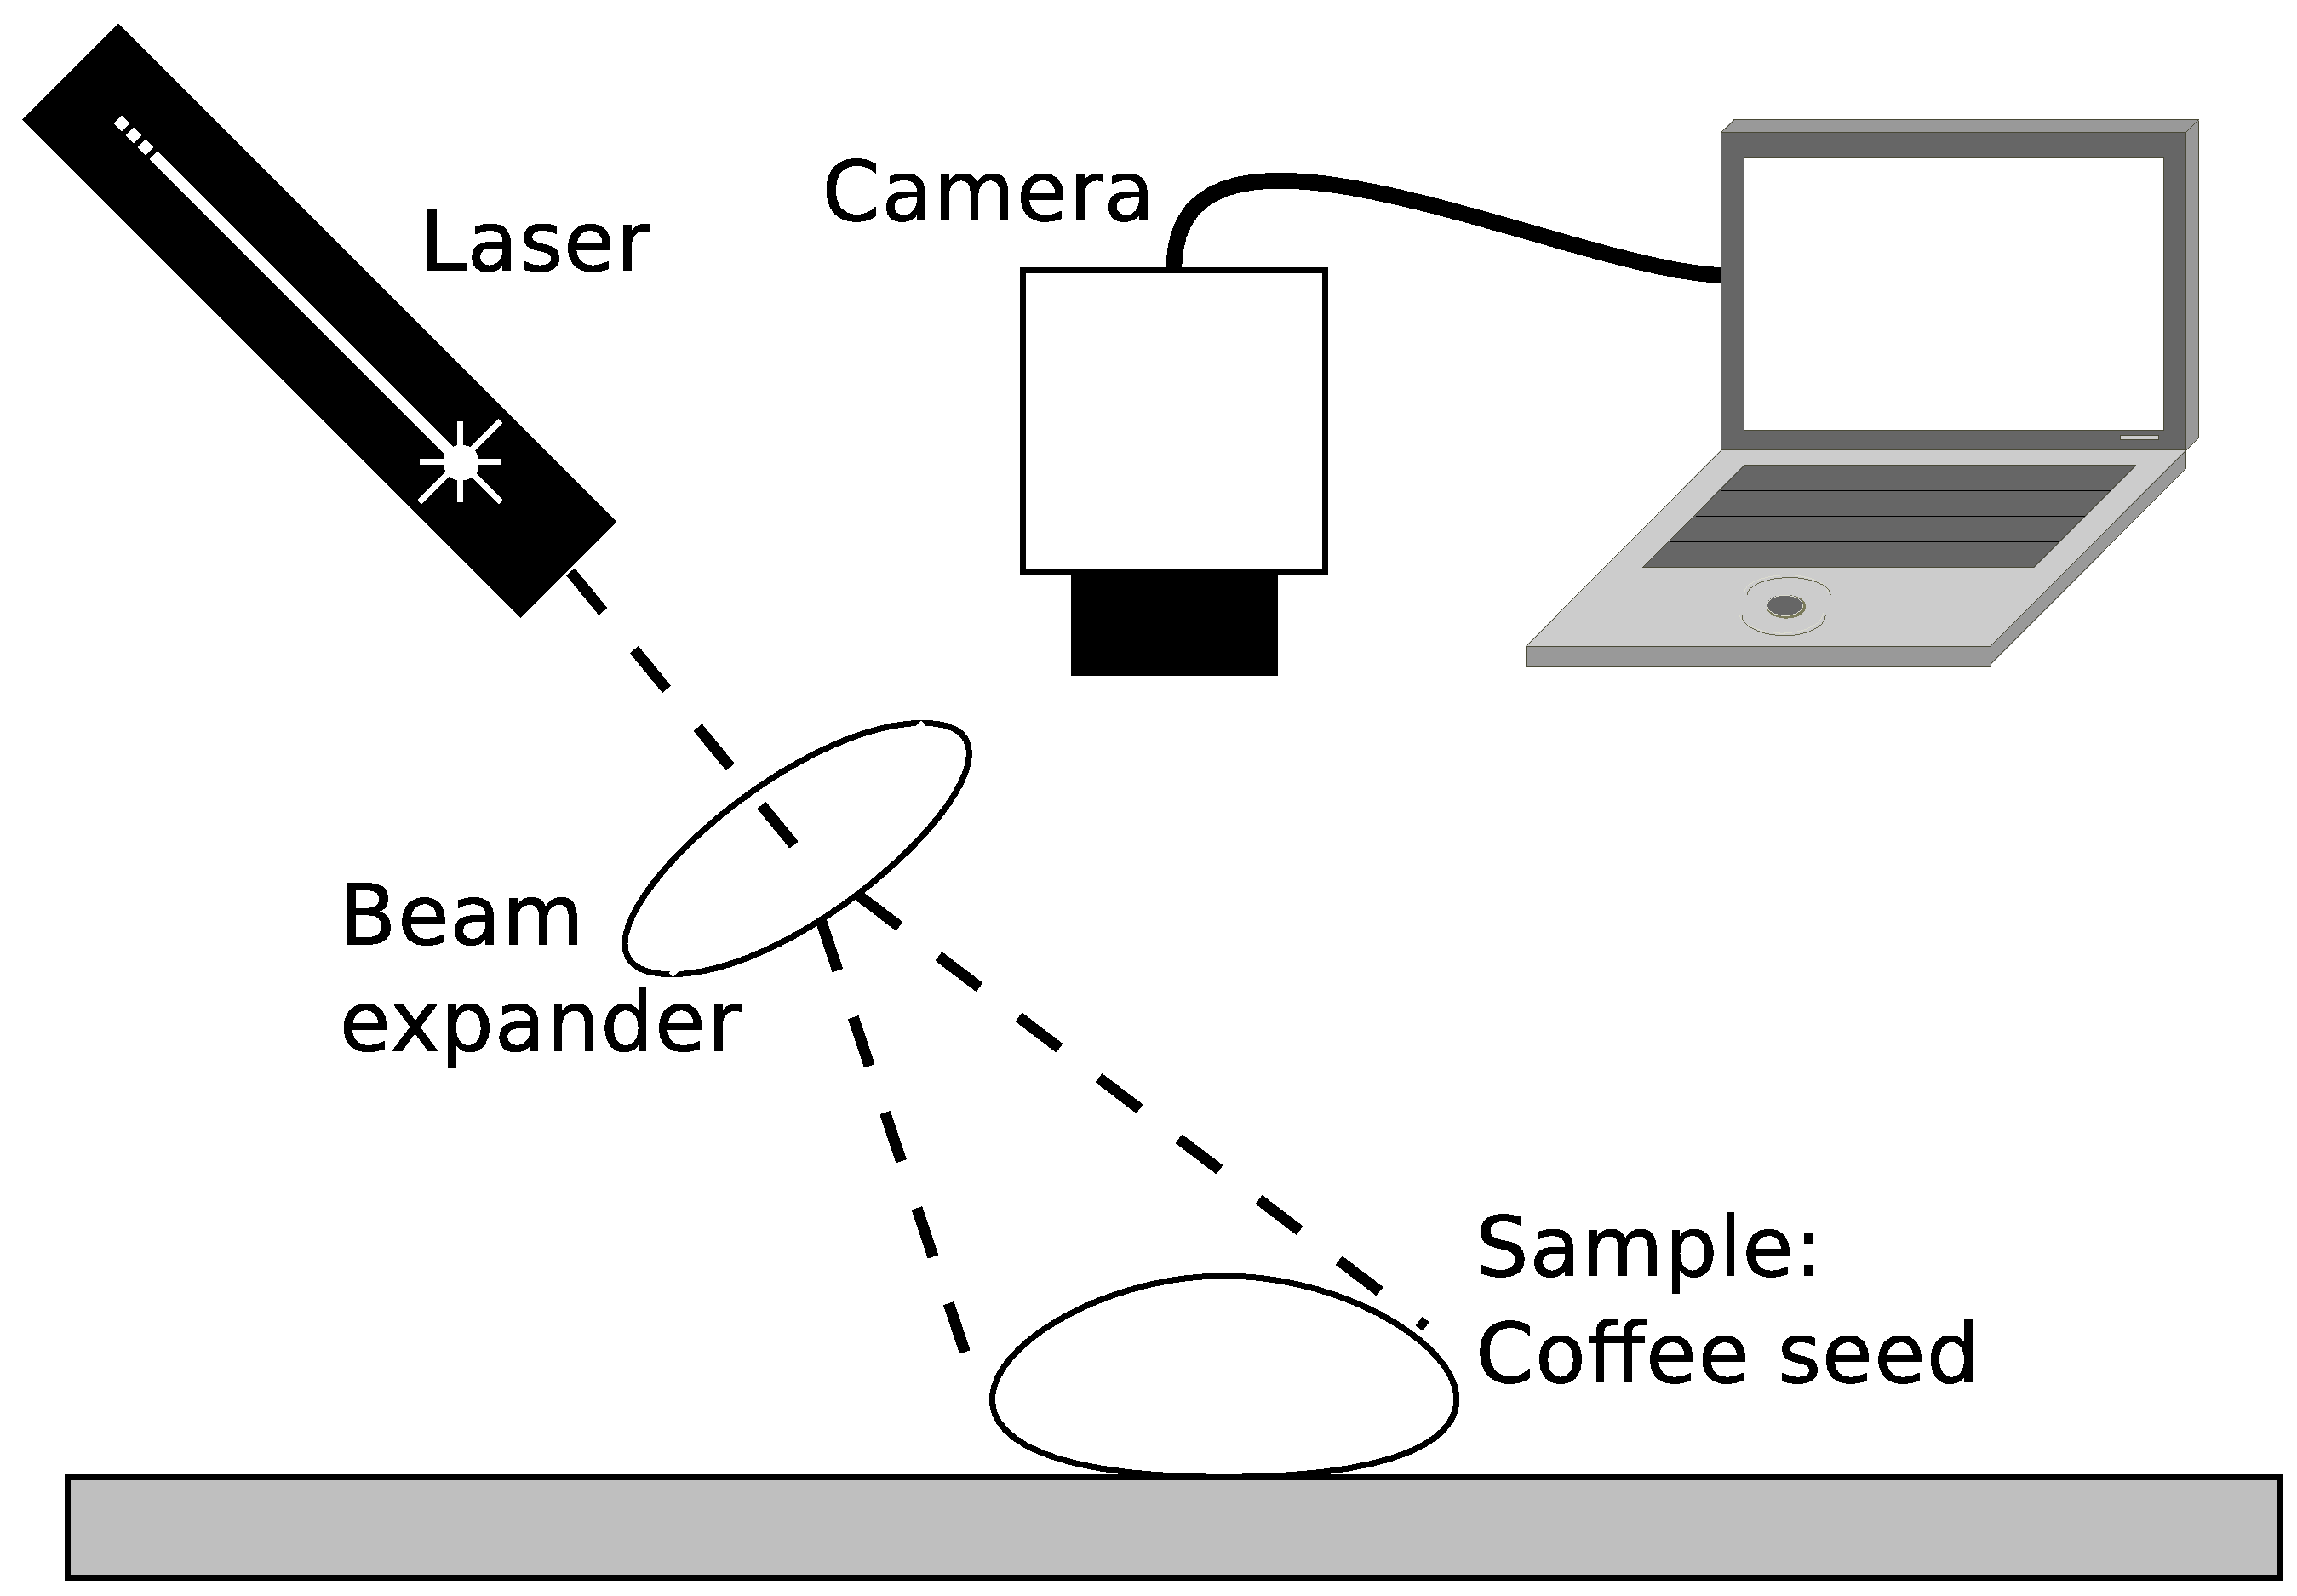
\includegraphics[width=0.55\columnwidth]{system.eps}
\caption{Data acquisition system setup of the coffee seed.  }
\label{fig:system}
\end{figure}
later the $M$ images are grouped in a data package (datapack).
Finally, it is in this point that will be apply the tests
aforementioned, and biospeckle indexes ($BSI$) are calculated 
in accordance with what is explained in the Secs. \ref{sec:soundsingleband} and \ref{sec:soundmultifreq}.


%%%%%%%%%%%%%%%%%%%%%%%%%%%%%%%%%%%%%%%%%%%%%%%%%%%%%%%%%%%%%%%%%%%%%%%%%%%%%%%%%%%%%%%%%
\section{Sound interpretation of a biospeckle index}
\label{sec:soundsingleband}
The Fig. \ref{fig:Diagrama0} represents the sound interpretation system diagram of a
biospeckle index; in it, we can see as is selected the $i$-th point set $S_i$, from a datapack,
and are processed to get any  biospeckle index known in the literature \cite{avd} \textcolor{blue}{[INDEX2] [INDEX3]}.
\begin{figure}[ht!]
\centering
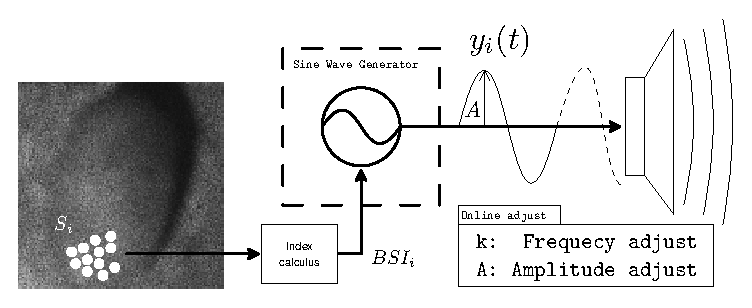
\includegraphics[width=0.99\columnwidth]{Diagrama0.eps}
\caption{Sound interpretation of a biospeckle index.}
\label{fig:Diagrama0}
\end{figure}
Thus, a biospeckle index value $BSI_i$ is obtained from $S_i$, and this information is sent to a sine wave generator
that fulfill the Eq. (\ref{eq:yisingleband}), 
\begin{equation}\label{eq:yisingleband}
 y_i= A~sin \left( 2 \pi f_i t \right),
\end{equation}
where, $A$ is the amplitude of sound that will be adjusted to suit the user, depending on your hearing level, 
$t$ is the elapsed time
and $f_i$ is the frequency of the wave, that is in function of $BSI_i$, see Eq. \ref{eq:fisingleband}.
\begin{equation}\label{eq:fisingleband}
 f_i= k~f_{ref}~\left( \frac{BSI_i}{BSI_{max}} \right)  
\end{equation}
where, $BSI_{max}$ is the maximum expected value of the used index, so that 
ever $\left( \frac{BSI_i}{BSI_{max}} \right) \leq 1$ , $f_{ref}$ is 
the reference frequency previously predefined by the user thereby $f_i$ ever be a portion 
of this value, and $k$ is a fine tuning value to $f_{ref}$ which will be
adjusted by the user. The last step of the diagram of Fig. \ref{fig:Diagrama0} shows
as the signal $y_i$ is played.
It is important to note, that to make the sound signal $y_i$ detected by the human ear, it should is in the 
audible spectrum \cite{humanrange}, this is $20 \leq f_i \leq 20khz $. But, some people
have a reduced audible range, and it is at this point that takes on 
importance the adjustment by $k$.

Finally, according the exposed, the Alg. \ref{alg:singleband} describe the procedure to make a 
sound interpretation of a $BSI$ in a single band system.


\begin{algorithm}
\SetKwInOut{Variables}{Variables}

 \KwData{A datapack $DATA$ with $M$ images.}
 \KwResult{The representation of a biospeckle index through a periodic sound.}
 $\circ$ Select the type of biospeckle index to be used;
 
 $\circ$ Choose the value of $f_{ref}$;
 
 $\circ$ $i \leftarrow 0$;

 ~\\
 \While{the user need,}{
  $\circ$ Select a point set $S_i$ in the datapack $DATA$;
  
  $\circ$ Calculate the biospeckle index $BSI_i$ over $S_i$;

  $\circ$ Evaluate $y_i$ according the Eqs. (\ref{eq:yisingleband}) and (\ref{eq:fisingleband}).
  
  $\circ$ Play the signal $y_i$ and adjust $k$ and $A$;
  
  $\circ$ $i \leftarrow i+1$;
  
  \If{Do you like exit}{
    break;
  }
 }
 \caption{Sound interpretation of a $BSI$ in a single band system.}
 \label{alg:singleband} 
\end{algorithm}



%%%%%%%%%%%%%%%%%%%%%%%%%%%%%%%%%%%%%%%%%%%%%%%%%%%%%%%%%%%%%%%%%%%%%%%%%%%%%%%%%%%%%%%%%
\section{Sound interpretation of a biospeckle index in a multi spectral analysis}
\label{sec:soundmultifreq}
To present an interpretation of a biospeckle index in a multi spectral analysis,
we need first to define the number and positions of the used frequency bands. Thus, the 
Fig. \ref{fig:Diagrama1a} represents an example case,
\begin{figure}[ht!]
\centering
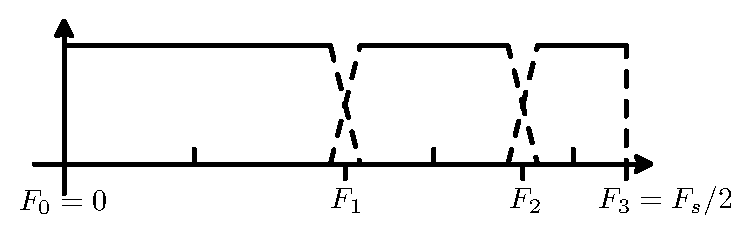
\includegraphics[width=0.6\columnwidth]{Diagrama1a.eps}
\caption{Separation of $N=3$ frequency bands in a multi spectral analysis.}
\label{fig:Diagrama1a}
\end{figure}
where 3 frequency bands are used. Given that, the images in datapack were sampled
with a frequency $F_s$; then, according the Nyquist theorem \cite{dsp}, 
the maximum signal frequency in the datapack is $F_s/2$. Additionally, we see
the values $F_j$, $\forall j \in \{1,2, ..., N\}$, that represent the cut-off frequency bands,
being $N$ the number of bands, with the special cases, $F_0=0$ and $F_N=F_s/2$.

The Fig. \ref{fig:Diagrama1} represents the sound interpretation system diagram of a
biospeckle index multi spectral analysis, using $N=3$ frequency bands.
\begin{figure}[ht!]
\centering
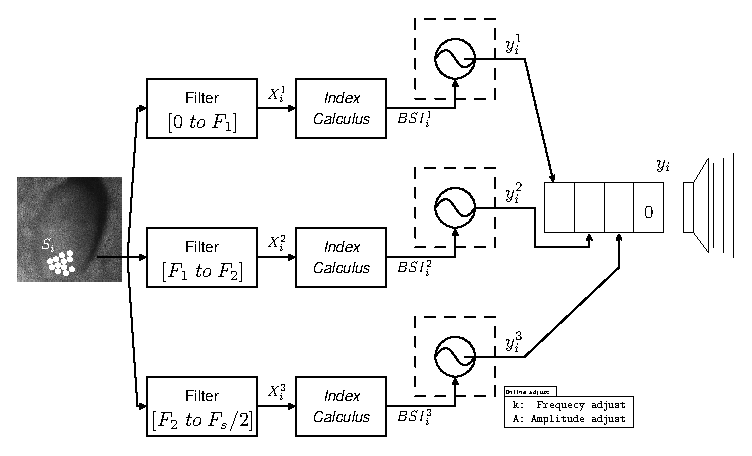
\includegraphics[width=0.99\columnwidth]{Diagrama1.eps}
\caption{Sound interpretation of a biospeckle index in a multi spectral analysis.}
\label{fig:Diagrama1}
\end{figure}
Similarly to the single band case, we can see as is selected the $i$-th point set $S_i$, from a datapack;
but now, the obtained signal is divided into bands. By example, in the Fig. \ref{fig:Diagrama1}
we have: A low frequency band from $0hz$ to $F_1$,
a middle frequency band from $F_1$ to $F_2$, and a high frequency band from $F_2$ to $F_s/2$;
later, over the signal $X_i^j$, in each band, they are calculated the biospeckle indexes 
$BSI^1_i$, $BSI^2_i$ and $BSI^3_i$, respectively. The indexes are sent to
sine wave generators with output $y^j_i$ as in the Eq. (\ref{eq:yjimultiband}),
\begin{equation}\label{eq:yjimultiband}
 y^j_i(t)= A~sin \left(2 \pi  f^j_{i} t \right),
\end{equation}
and later these signals are grouped in a new signal $y^j_i$ like seen in the Fig. \ref{fig:Diagrama2};
\begin{figure}[ht!]
\centering
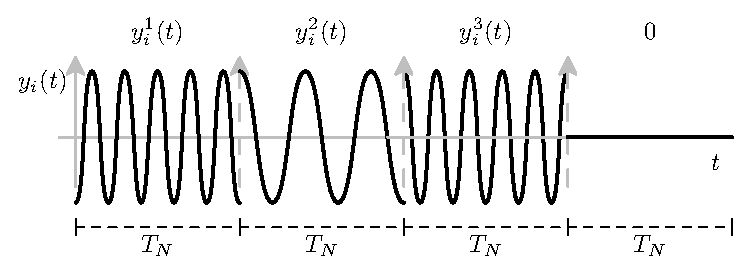
\includegraphics[width=1.0\columnwidth]{Diagrama2.eps}
\caption{Signal $y_i(t)$ formed by grouping $T_N$ seconds of signals $y^1_i(t)$, $y^2_i(t)$ and $y^3_i(t)$ with $T_N$ seconds of zero samples at end.}
\label{fig:Diagrama2}
\end{figure}
where, $i$ represents the used point set, $j$ represents the used frequency band,
$A$ is the amplitude of sound that will be adjust to suit the user, $t$ is the elapsed time
and $f^j_i$ is in function of $BSI^j_i$, as
can be see in the Eq. (\ref{eq:fjimultiband}),
\begin{equation}\label{eq:fjimultiband}
 f^j_{i}=k~f_{ref}~\left( \frac{BSI^j_i}{BSI_{max}} \right),
\end{equation}
where, $BSI_{max}$ is the maximum expected value of the used biospeckle index in all frequency bands, so that 
ever $\left( \frac{BSI^j_i}{BSI_{max}} \right) \leq 1$ and
$f_{ref}$ is the reference frequency, it should be selected by the user and should be less than $f_s/2$, being $f_s$
the sampling frequency of digital sound synthesizer.
Finally the sound signals $y^j_i(t)$ are grouped and the resulted signal $y_i(t)$ is played, see Eq. (\ref{eq:yiendmultiband}),
\begin{equation}\label{eq:yiendmultiband}
 y_i(t)= \sum_j \varPi\left(t-(j-1)~T_N\right) y^j_i(t);
\end{equation}
where, $\varPi\left(t\right)$ is a rectangular function of size $T_N$.
The Alg. \ref{alg:multiband} shows the procedure explained above.

\begin{algorithm}
\SetKwInOut{Variables}{Variables}

 \KwData{A datapack $DATA$ with $M$ images.}
 \KwResult{The  representation of biospeckle indexes in a multi band system, through a periodic sound.}
 $\circ$ Select the type of biospeckle index to be used;
  
 $\circ$ Choose the  sampling frequency $f_s$ of digital sound synthesizer;
 
 $\circ$ Choose the cut-off values $F_j$ of the frequency bands;
 
 $\circ$ $i \leftarrow 0$;
 ~\\
 \While{the user need,}{
  $\circ$ Select a point set $S_i$ in the datapack $DATA$;
  
  $\circ$ Filter $\forall j$, the information in $S_i$ and return the signals $X_i^j$;
  
  $\circ$ Calculate $\forall j$, the biospeckle index $BSI^j_i$ from $X_i^j$;

  $\circ$ Evaluate $\forall j$, $y^j_i$ according the Eqs. (\ref{eq:yjimultiband}) and (\ref{eq:fjimultiband}).
  
  $\circ$ Play the signal $y_i$ according the Eq. (\ref{eq:yiendmultiband}) and adjust $k$ and $A$;
  
  $\circ$ $i \leftarrow i+1$;
  
  \If{Do you like exit}{
    break;
  }
 }
 \caption{Sound interpretation of a $BSI$ in a multi band system.}
 \label{alg:multiband} 
\end{algorithm}

%%%%%%%%%%%%%%%%%%%%%%%%%%%%%%%%%%%%%%%%%%%%%%%%%%%%%%%%%%%%%%%%%%%%%%%%%%%%%%%%%%%%%%%%%
%%%%%%%%%%%%%%%%%%%%%%%%%%%%%%%%%%%%%%%%%%%%%%%%%%%%%%%%%%%%%%%%%%%%%%%%%%%%%%%%%%%%%%%%%
\section{Numerical results} 
\label{sec:numerical}

\subsection{Numerical results of single band test} 
\label{subsec:numericalsingle}
To made a single band test will be used the (normalized) $AVD$ biospeckle index \cite{avd},
according the system diagram showed in the Fig. \ref{fig:Diagrama0}. Thus,
over the datapack are selected 3 point set (red points, blue points and green points) with 
$200$ points (pixels) each one, being these randomly chosen in the space using a Gaussian probability distribution 
with radius of $15$ pixels, 
as can be seen in the Fig. \ref{fig:select_points_avd}.
\begin{figure}[ht!]
\centering
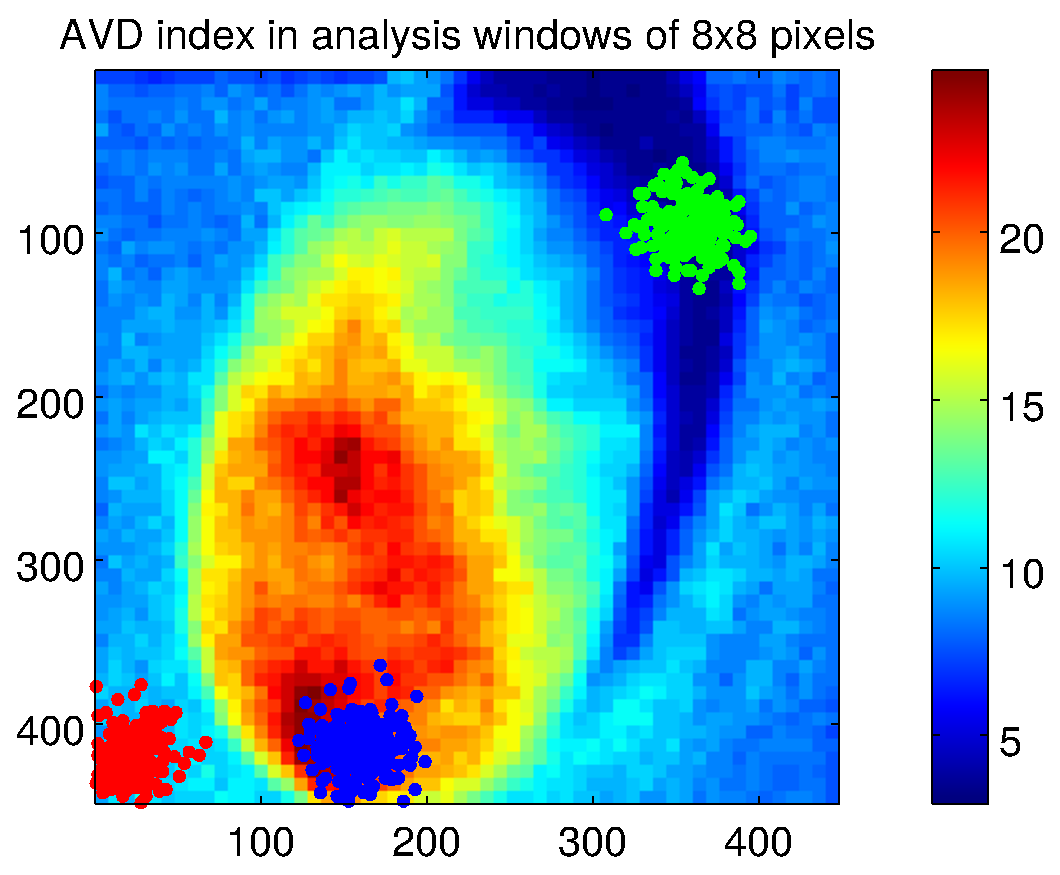
\includegraphics[width=0.5\columnwidth]{select_points_avd.eps}
\caption{Selecting the points to be analyzed.}
\label{fig:select_points_avd}
\end{figure}
To facilitate the selection of points and the interpretation of the results, 
the point sets were chosen over an image that represent the $AVD$ values in graphic mode \cite{BSLTLBOOK},
calculated over all the points (pixels) contained in analysis windows of $8 \times 8$ pixels,
the relation between the colors and the $AVD$ values is expressed by a color bar.
Thus, the $AVD$ values of the set points are according the Tab. \ref{tab:1}, it is easy to see
that it match with the data seen in the Fig. \ref{fig:select_points_avd}.
\begin{table}[!hbt]
\caption{$AVD$ values in the point sets.}
\begin{center}
\begin{tabular}{|l |l | l | l |}
\hline
   ~               & Red points ($i=1$) & Blue points ($i=2$) & Green points ($i=3$) \\
\hline
\hline
$AVD_i$              & $10.06$   & $21.41$    & $3.70$ \\
\hline
$AVD_i~\frac{2}{255}$ & $0.079$   & $0.168$    & $0.029$ \\
\hline
\end{tabular}
\end{center}
\label{tab:1}
\end{table}
Now, according the seen in the Sec. \ref{sec:soundsingleband} in the 
Eqs. (\ref{eq:yisingleband}) and (\ref{eq:fisingleband}), the $AVD$ biospeckle
indexes are interpreted, using the values $A=1.0$, $k=4.0$ and $f_{ref}=f_s/2$,
being that $f_s$ is the sampling frequency of synthesized sound $y_i$. Thus,
the final sound has a signal with a form as in the Eqs. (\ref{eq:yisinglebandT1})
and (\ref{eq:fisinglebandT1}),
\begin{equation}\label{eq:yisinglebandT1}
 y_i= sin \left( 2 \pi f_i t \right),
\end{equation}
\begin{equation}\label{eq:fisinglebandT1}
 \frac{f_i}{f_s}=  AVD_i~\frac{2}{255}.
\end{equation}
The Fig. \ref{fig:image-freq-single} shows, the frequency space behavior of the
signals $y_i$, being the red, blue and green point represented by $y_1$, $y_2$ and $y_3$ 
respectively; the graphic was created using the Fourier transform and exemplify
as the fundamental frequency of signal $y_i$ change of value in accordance to $AVD_i$
and following the Tab. \ref{tab:1}.
\begin{figure}[ht!]
\centering
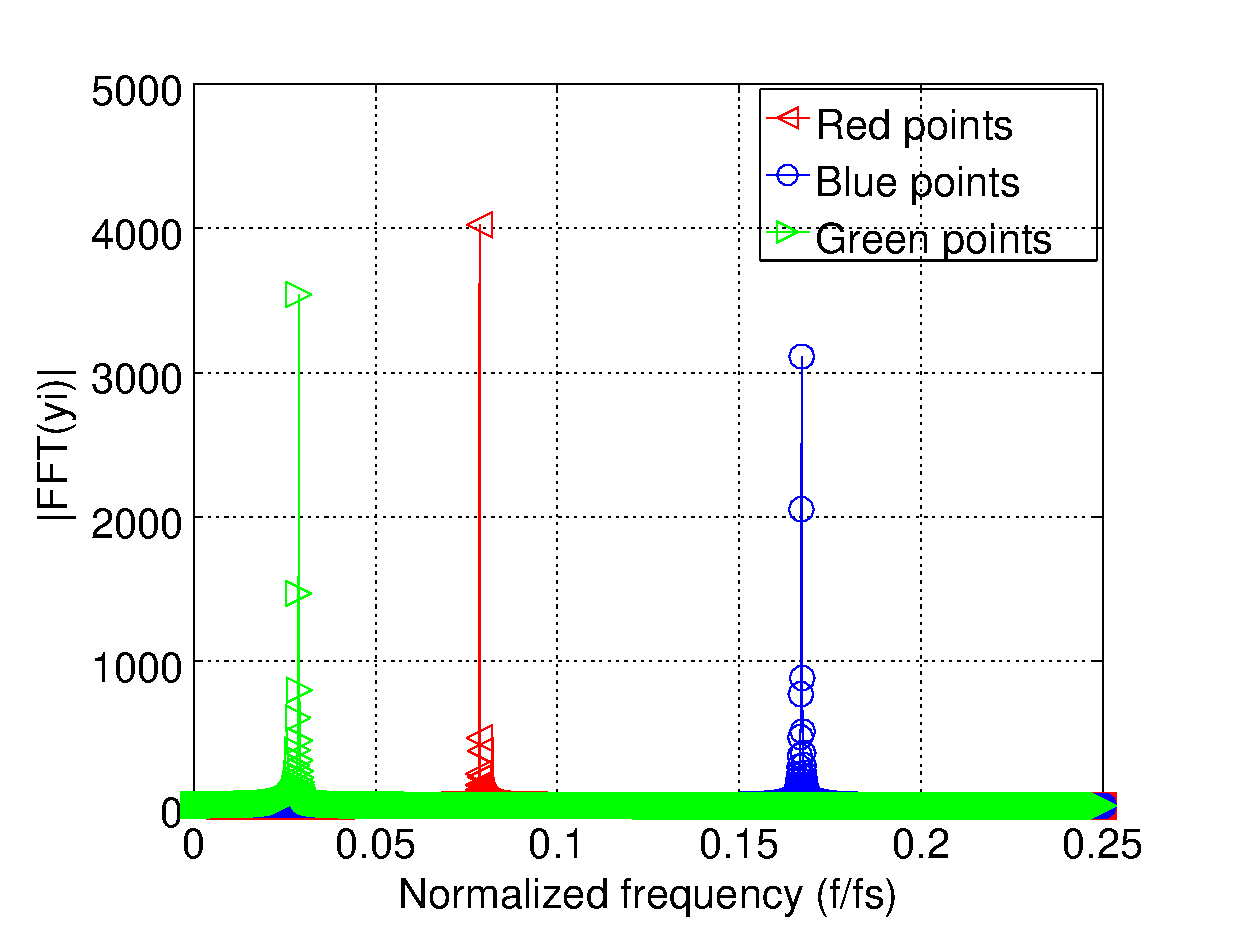
\includegraphics[width=0.5\columnwidth]{image-freq-single.eps}
\caption{Frequencies of the signals $y_i$ obtained.}
\label{fig:image-freq-single}
\end{figure}

The audio files: ``$audio-single1.wav$'', ``$audio-single2.wav$'' and ``$audio-single3.wav$''; 
with the sound interpretations calculated using the Eqs. (\ref{eq:yisinglebandT1}) 
and (\ref{eq:fisinglebandT1}); from the point sets red, blue and green respectively; 
they can be downloaded from an on-line repository \textcolor{blue}{FALTA SITE $>>>>$} \cite{BSLTLSINGLE}.


%%%%%%%%%%%%%%%%%%%%%%%%%%%%%%%%%%%%%%%%%%%%%%%%%%%%%%%%%%%%%%%%%%%%%%%%%%%%%%%%%%%%%%%%%
\subsection{Numerical results of multi band test} 
\label{subsec:numericalmulti}
To made a biospeckle multi-band test will be used the temporal standard deviation biospeckle 
index \cite{Nothdurft:05}, apply to all point set  $S_i$, selected 
according the system diagram showed in the Fig. \ref{fig:Diagrama1}, where $i$ is the indexer
of selected point set. Thus,
over the datapack are selected 3 point sets ($S_1$ red points, $S_2$ blue points and $S_3$ green points) with 
$200$ points (pixels) each one. The same way, that in the single band test, in the multi-band test
the points were randomly chosen in the space, using a Gaussian probability distribution 
with a radius of $15$ pixels, see Fig. \ref{fig:select_points_std}.
\begin{figure}[ht!]
\centering
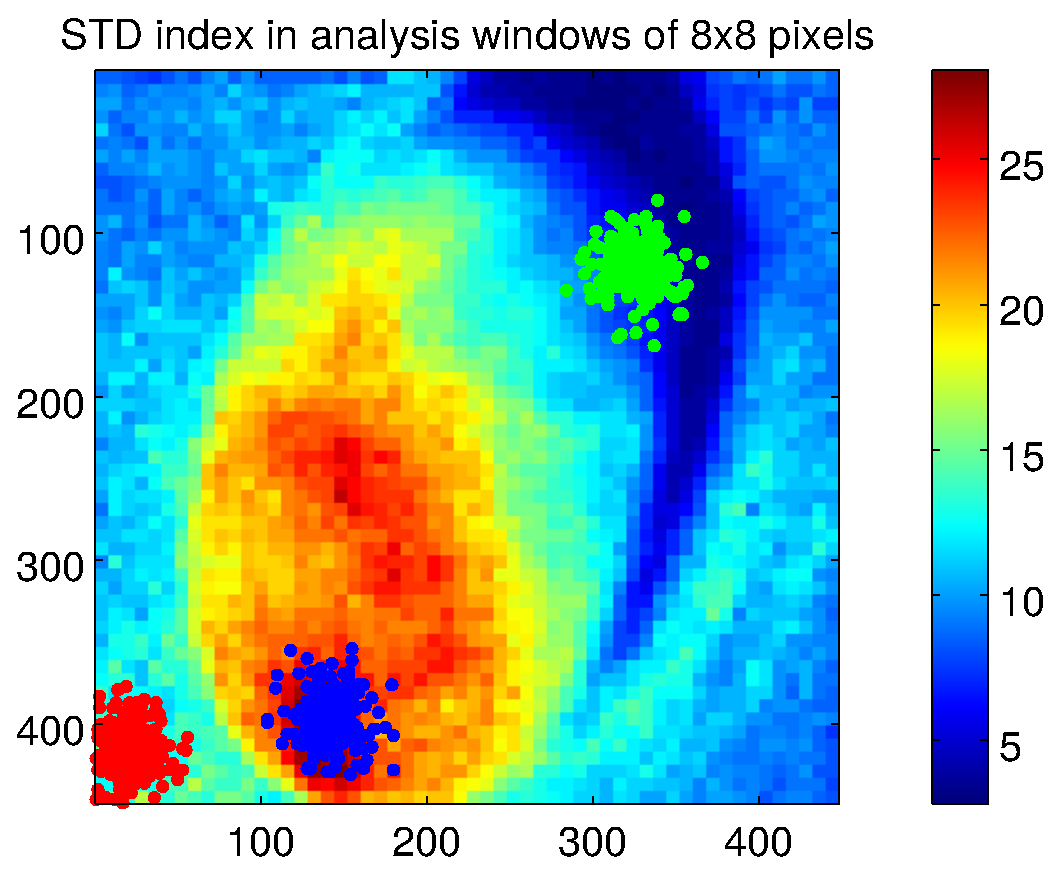
\includegraphics[width=0.5\columnwidth]{select_points_std.eps}
\caption{Selecting the points to be analyzed in the biospeckle multi-band test.}
\label{fig:select_points_std}
\end{figure}
In this case the selection of points were made over an image that represents 
the temporal standard deviation in graphic mode \cite{BSLTLBOOK,Nothdurft:05},
where it was made with analysis windows of $8 \times 8$ pixels;
the relation between the colors and the temporal standard deviation biospeckle 
index values is expressed by a color bar.

As explicated in the Figs. \ref{fig:Diagrama1a} and \ref{fig:Diagrama1}, each point set $S_i$ was separated
in $3$ frequency bands; thus, in this test, the values of cut-off frequencies will be
$F_0=0$, $F_1=\frac{3}{9}\frac{F_s}{2}$, $F_2=\frac{6}{9}\frac{F_s}{2}$ and $F_3=\frac{F_s}{2}$, being that
the sampling frequency of images in the datapack was $F_s=12.5~hz$. Thereby, 
the signals $X^1_i$, $X^2_i$ and $X^3_i$ were obtained from the bands $\{F_0 \rightarrow F_1\}$,
$\{F_1 \rightarrow F_2\}$ and $\{F_2 \rightarrow F_3\}$ respectively; over these signals 
are calculated by each one a temporal standard deviation biospeckle index, being these
$BSI^1_i$, $BSI^2_i$ and $BSI^3_i$, the values obtained can be seen in the Tab \ref{tab:2}.

\begin{table}[!hbt]
\caption{$STD$ values in the frequency bands by point sets.}
\begin{center}
\begin{tabular}{|l |l | l | l |}
\hline
   ~               & $BSI^1_i$ & $BSI^2_i$ & $BSI^3_i$ \\
\hline
\hline
Red points   ($i=1$)&   13.4739&    7.3840&    6.6311\\
Blue points  ($i=2$)&   20.4776&   12.6959&   11.8572\\
Green points ($i=3$)&    5.2657&    3.6161&    3.5850\\
\hline
\end{tabular}
\end{center}
\label{tab:2}
\end{table}
Finally, using the values $A=1.0$ and $k=1.0$ were obtained all the signals 
$y^j_i$ and these were processed according the Eq. (\ref{eq:yiendmultiband})
to get the signals $y_1$, $y_2$ and $y_3$, representing these to the point sets $S_1$, $S_2$ and $S_3$,
respectively; as can be seen in the Figure \ref{fig:yfuncs}.
\begin{figure}[ht!]
\centering
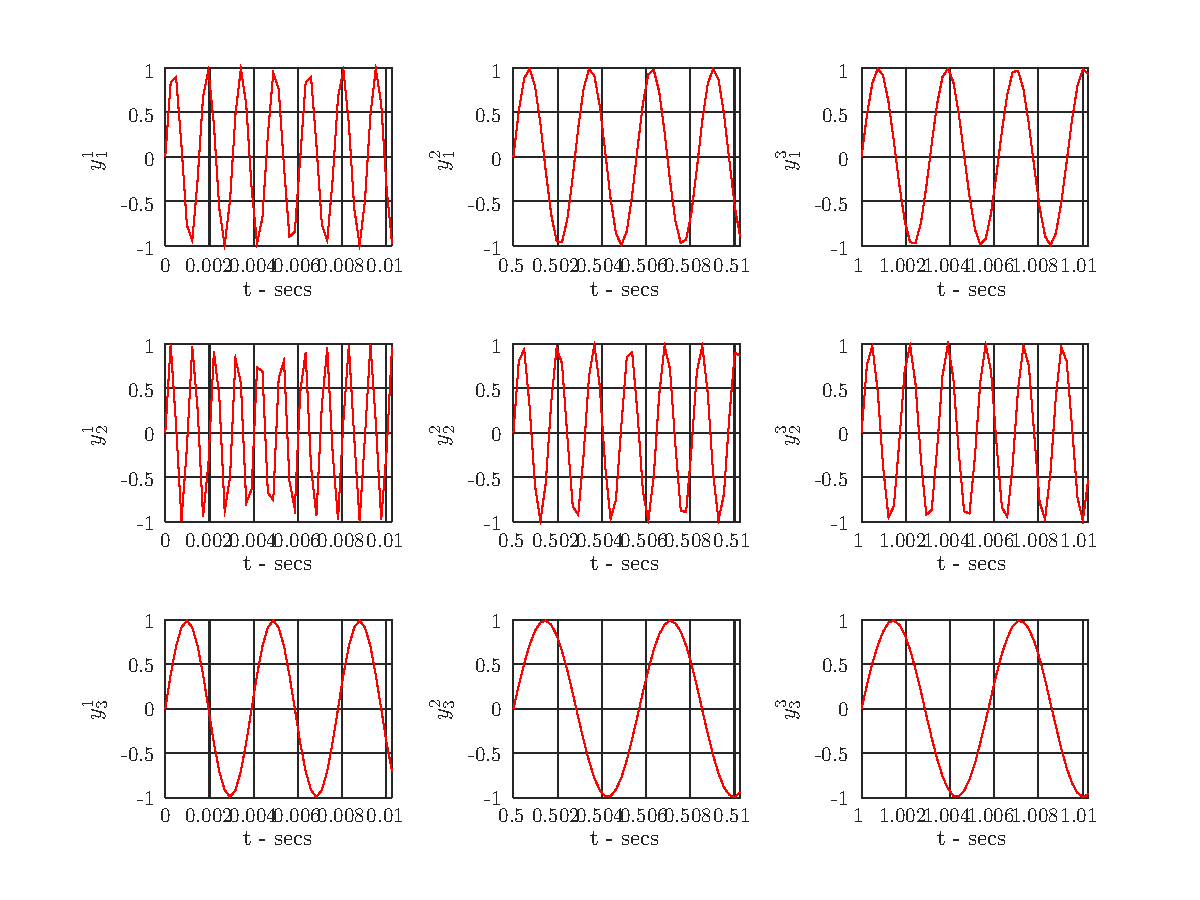
\includegraphics[width=0.99\columnwidth]{yfuncs.eps}
\caption{Signals $y_i(t)$ to the 3 point sets.}
\label{fig:yfuncs}
\end{figure}
Thus, listening the sound interpretation of the signals $y_1$, $y_2$ and $y_3$, it is easy
identify subjectively the level of biospeckle index.
The sound files contain these data are the next: 
``$audio-multi1.wav$'', ``$audio-multi2.wav$'' and ``$audio-multi3.wav$''; 
they represents the point sets red, blue and green respectively; 
and they can be downloaded from an on-line repository \textcolor{blue}{FALTA SITE $>$} \cite{BSLTLMULTI}.
Additionally, in the same audio files, the 3 frequency bands can be analyzed subjectively the level
of biospeckle activity, given the human brain is specialized in differentiating sounds of different frequencies.

%%%%%%%%%%%%%%%%%%%%%%%%%%%%%%%%%%%%%%%%%%%%%%%%%%%%%%%%%%%%%%%%%%%%%%%%%%%%%%%%%%%%%%%%%
%%%%%%%%%%%%%%%%%%%%%%%%%%%%%%%%%%%%%%%%%%%%%%%%%%%%%%%%%%%%%%%%%%%%%%%%%%%%%%%%%%%%%%%%%
\section{Distinction of activity level using the biospeckle index} 
Given that the perception of biospeckle activity using a sound, it is linked to the possibility
of distinct between two phenomenon through the comparison between two different levels of the biospeckle index. 
Then, the next test shows this behavior comparing the $std$ biospeckle index of 8 dead seeds
with 8 alive seeds, the samples were collected around the radicle of seeds, using $200$ points 
randomly selected using a Gaussian distribution with 15 pixel of radius. In all case the signals
were processed, so that each one was subdivide in three frequency bands, like in the 
Sec. \ref{subsec:numericalmulti}. Thereby, we obtain the results shown in the Figs. \ref{fig:DATA00-STD-box},
\ref{fig:DATA01-STD-box} and \ref{fig:DATA1-STD-box}, that represent the $std$ biospeckle index
of signals in the bands $0$ to $F_1$, $F_1$ to $F_2$ and $F_2$ to $F_s/2$, respectively.

\begin{figure}[ht!]
\centering
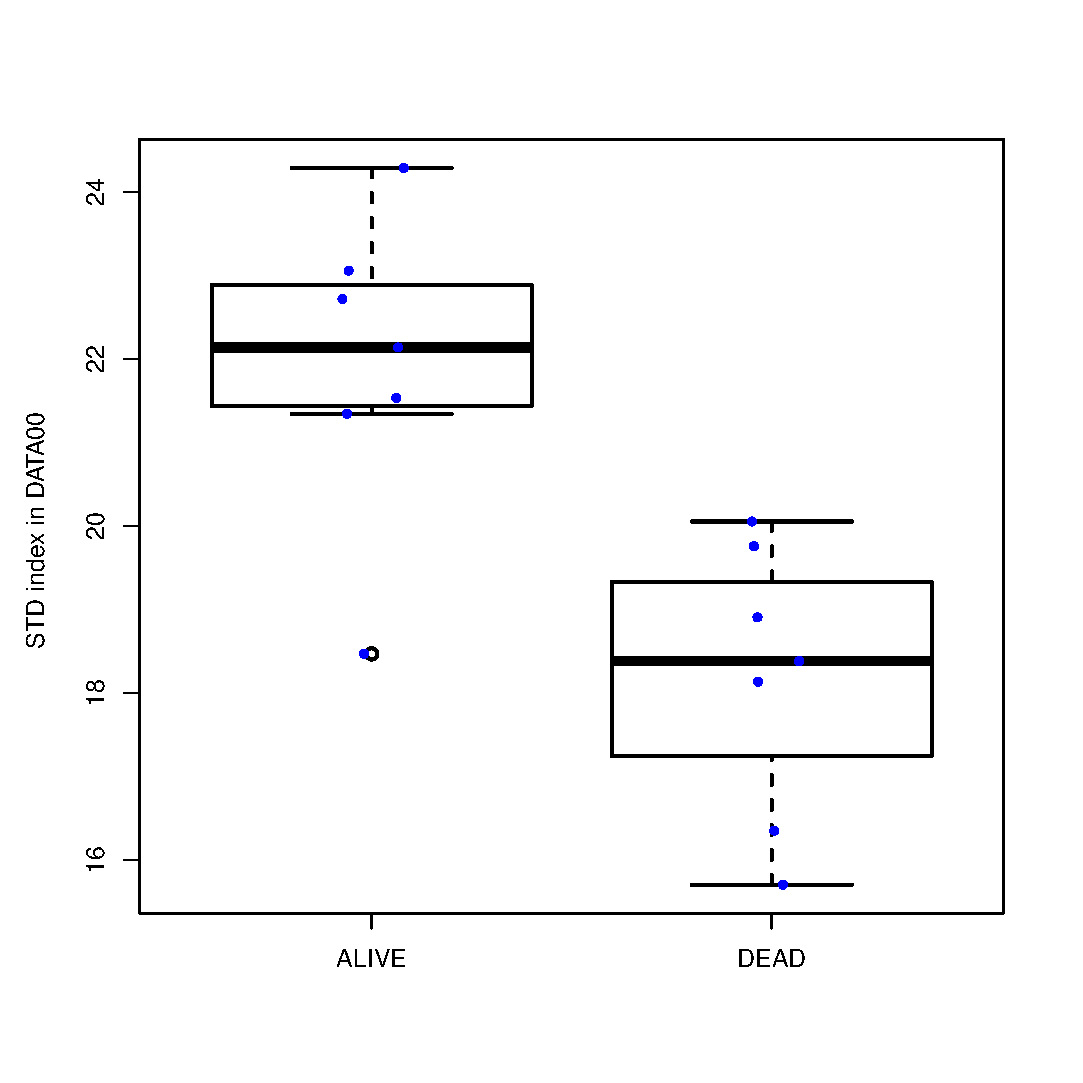
\includegraphics[width=0.6\columnwidth]{DATA00-STD-box.eps}
\caption{Std index values, of signals between $0$ and $F_1$ hz, in the radicle of 16 dead and alive seeds.}
\label{fig:DATA00-STD-box}
\end{figure}

\begin{figure}[ht!]
\centering
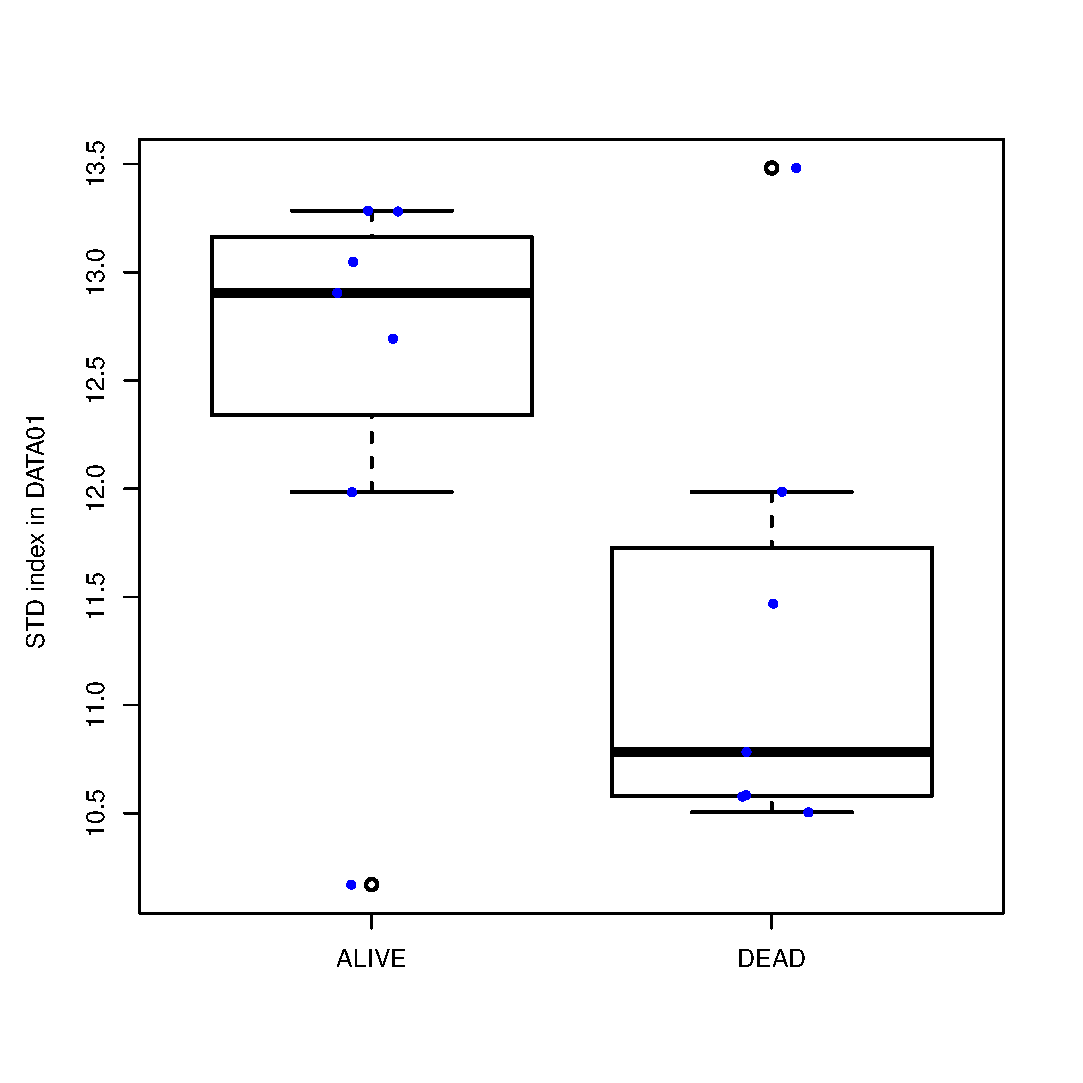
\includegraphics[width=0.6\columnwidth]{DATA01-STD-box.eps}
\caption{Std index values, of signals between $F_1$ and $F_2$ hz, in the radicle of 16 dead and alive seeds.}
\label{fig:DATA01-STD-box}
\end{figure}

\begin{figure}[ht!]
\centering
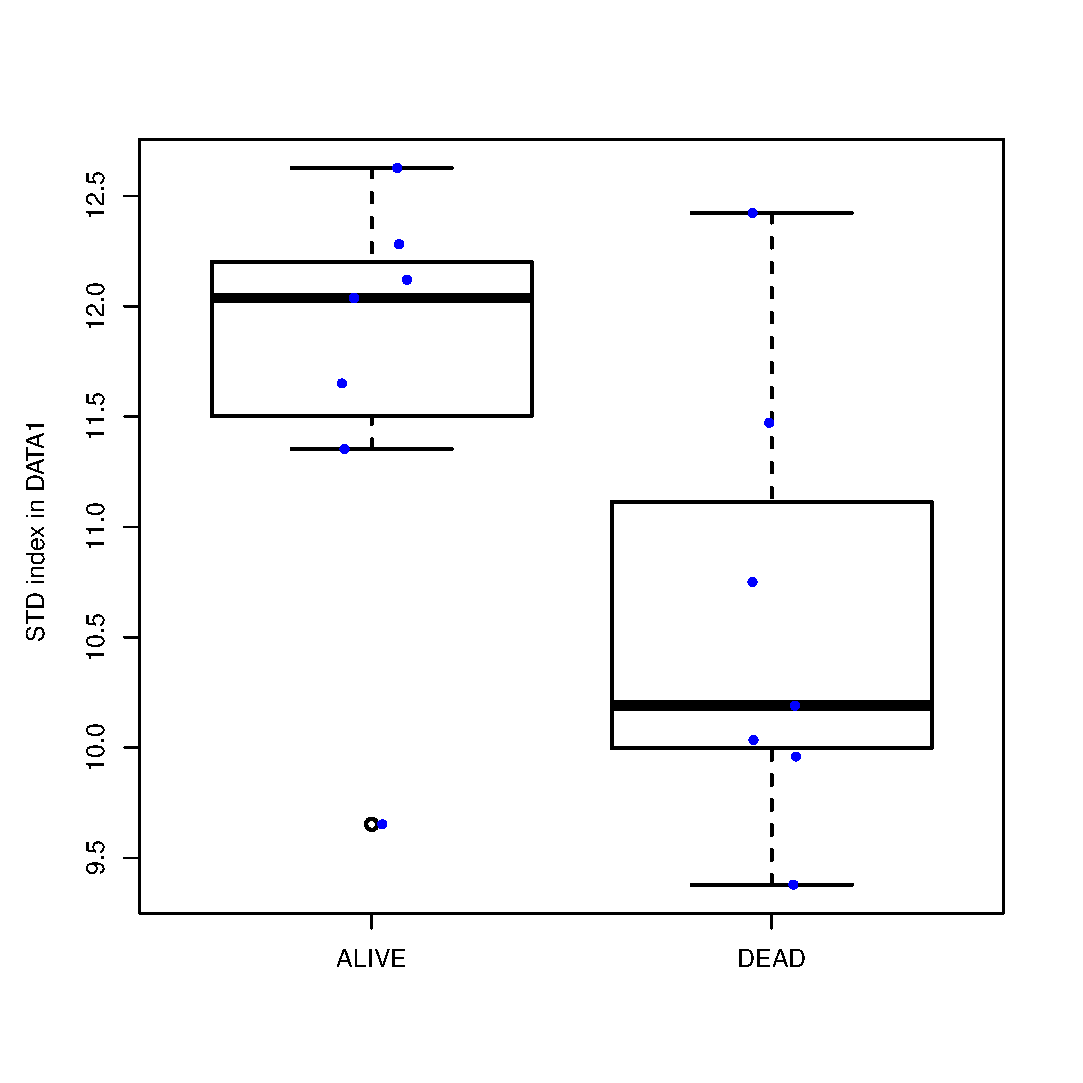
\includegraphics[width=0.6\columnwidth]{DATA1-STD-box.eps}
\caption{Std index values, of signals between $F_2$ and $F_s/2$ hz, in the radicle of 16 dead and alive seeds.}
\label{fig:DATA1-STD-box}
\end{figure}

It is easy to see that exist different separation levels of the value of biospeckle indexes, depending
of the analyzed frequency band; in the test, the band where exist a greater degree of separation it
is between $0$ and $F_1$ hz. Given that, an alive seed have a biospeckle index value around $22$
and a dead seed a value around $18$, it is important to note that it is a statistic analysis
and consequently exist samples that not fulfill a pattern, like the sample of alive seed
with a lower std value of $18.5$, see Fig. \ref{fig:DATA00-STD-box}. 

For the above, it is important to note that the technique of to use a sound as
a qualitative index, should consider the sensibility level of human ear
to distinguish between two frequencies, considering that this configuration
also should be influenced by the analyzed frequency band.

%%%%%%%%%%%%%%%%%%%%%%%%%%%%%%%%%%%%%%%%%%%%%%%%%%%%%%%%%%%%%%%%%%%%%%%%%%%%%%%%%%%%%%%%%
%%%%%%%%%%%%%%%%%%%%%%%%%%%%%%%%%%%%%%%%%%%%%%%%%%%%%%%%%%%%%%%%%%%%%%%%%%%%%%%%%%%%%%%%%
\section{Conclusion} 

In this work were presented two  methods to the sound interpretation of biospeckle analysis.

The first method analyze the biospeckle signal using a single frequency band model, 
in this case was showed through of a numerical analysis that the representation 
using an unique wave form, in this case a sound sine wave, it is efficient; and that the variation
of the biospeckle index used can be easily represented and perceived by the frequency variation of sine wave,
being it a good tool to a fast  biospeckle subjective  analysis.


By other side, in the second method, with a multi frequency band approach,
it was necessary to assign to each frequency band a different wave form pattern $g^i(f)$,
so that the variations of biospeckle index in each band will be linked to repetition frequency variation
of the  wave form pattern. This method also shown be efficient to identify  subjectively
the variation of a biospeckle index in a determined frequency band.

\section{Acknowledgment}
We wish to acknowledge the partial financial support for this study provided by the $CAPES$ 
scholarship
$PNPD$ Program, $FAPEMIG$ and $CNPQ$.

%----------------------------------------------------------------------------------------
%	REFERENCE LIST
%----------------------------------------------------------------------------------------
\section{Bibliography}
\bibliography{report}   %>>>> bibliography data in report.bib
\bibliographystyle{spiebib}   %>>>> makes bibtex use spiebib.bst


%----------------------------------------------------------------------------------------

\end{document} 
